% Versão em português, explicada, do relatório da Task 1 (só para estudo do Rodrigo).
% NÃO é para entregar: o relatório oficial é relatorio_task1.tex (inglês, IEEE, 2 páginas).
% Os números são os mesmos do relatório oficial e de task1/analise_resultados_t1.txt.
\documentclass[11pt,a4paper]{article}
\usepackage[utf8]{inputenc}
\usepackage[margin=2.2cm]{geometry}
\usepackage{float}
\usepackage{graphicx,booktabs,amsmath,xcolor,enumitem,array}
\usepackage[hidelinks]{hyperref}
\renewcommand{\figurename}{Figura}
\renewcommand{\tablename}{Tabela}
\renewcommand{\contentsname}{Índice}
\setlist{itemsep=2pt,topsep=3pt}
\setlength{\parskip}{4pt}
\newcommand{\porque}[1]{\par\noindent\colorbox{blue!6}{\parbox{\dimexpr\linewidth-2\fboxsep}{\small\textbf{Porquê?} #1}}\par}
\newcommand{\cuidado}[1]{\par\noindent\colorbox{orange!10}{\parbox{\dimexpr\linewidth-2\fboxsep}{\small\textbf{Atenção.} #1}}\par}

\sloppy
\begin{document}
\begin{center}
{\LARGE\bfseries Task 1 explicada em português}\\[4pt]
{\large Caracterização do Deucalion para o Jacobi 3D \emph{varcoef}}\\[4pt]
Versão de estudo para o Rodrigo, 21/11/2026. Não é para entregar.
\end{center}

\noindent Este documento conta, em português e com calma, o que está no relatório oficial
(\texttt{relatorio\_task1.pdf}, em inglês e com 2 páginas). Os números são exatamente os mesmos.
A diferença é que aqui se explica \emph{de onde vem} cada número, \emph{porque} tomámos cada decisão e
o que correu mal pelo caminho. As caixas azuis respondem ao ``porquê?'' e as laranja assinalam
armadilhas.

\tableofcontents

\section{A ideia geral em 1 minuto}
A Task 1 pede para conhecermos as máquinas \emph{antes} de otimizar o código. Para isso:
\begin{enumerate}
\item \textbf{1.1:} medir o que cada partição do Deucalion (x86, ARM e A100) consegue fazer, ou seja, a
velocidade de cálculo, a velocidade da memória e o atraso da memória.
\item \textbf{1.2:} desenhar o \emph{roofline} do AMD e do A64FX no mesmo gráfico.
\item \textbf{1.3:} acrescentar ``tetos'' que digam o que acontece se o código não usar bem a máquina.
\item \textbf{1.4:} planear como vamos medir tudo na Task 2.
\end{enumerate}
As três grandes lições, que também estão no \emph{abstract}, foram estas:
\begin{itemize}
\item o clock real do AMD sob carga põe o pico 22\% \emph{acima} do valor do catálogo;
\item no A64FX uma divisão é 393 vezes mais lenta do que o pico de cálculo, e o nosso algoritmo tem 7 divisões por ponto;
\item se a memória ficar toda num só nó NUMA, a banda cai 7 a 10 vezes.
\end{itemize}

\section{O algoritmo: o que o \emph{varcoef} faz e porque isso importa}
O \emph{varcoef} resolve a equação do calor num material com 4 materiais diferentes. Cada ponto da
grelha 3D é atualizado com a média dos 6 vizinhos (stencil de 7 pontos). A ``condutividade'' entre dois
pontos vizinhos $p$ e $q$ é uma \textbf{média harmónica}:
\[
\kappa_{pq} = \frac{2\,k_p k_q}{k_p + k_q}
\]
Cada uma das 6 médias harmónicas tem uma divisão, e há mais uma divisão no fim, para normalizar.
Ficam \textbf{7 divisões por ponto}, e o código de referência fá-las em \texttt{double}.

\textbf{Contagem de operações (FLOP).} Somando as multiplicações, somas e divisões, dá cerca de
\textbf{45 FLOP por ponto}. O resíduo acrescenta 3, por isso uma iteração completa tem 48.

\textbf{Contagem de bytes.} O ciclo principal (o \emph{sweep}) lê \texttt{u} (4 B, float), lê o material
(4 B, porque a referência o guarda em \texttt{int}) e escreve \texttt{u\_new} (4 B). São
\textbf{12 bytes úteis por ponto}.

\textbf{Intensidade aritmética (OI).} É a razão entre FLOP e bytes: $45/12 = 3.75$ FLOP/B no sweep. Na
iteração completa, que inclui o resíduo e a cópia de volta para \texttt{u}, são 48 FLOP para 28 B úteis,
ou seja 1.71 FLOP/B.

\porque{Contamos bytes \emph{úteis} (sem o write-allocate) por causa da decisão D24. O tráfego extra
(write-allocate e linhas meio usadas) aparece nos \emph{tetos} M1 e M3, que são bandas mais baixas.
Se o contássemos também na OI, contávamos o mesmo custo duas vezes.}

\textbf{Motivação (D27).} A introdução do relatório oficial termina com esta frase: \emph{``Datasheet
peaks hide this kernel's real limits (divisions, strides, NUMA), so we measure each one before optimising
in Task~2.''} Em português: os picos do catálogo escondem os limites reais deste algoritmo, que são as
divisões, o stride e o NUMA. Por isso medimos cada um antes de otimizar.
\porque{É a resposta curta a ``porque é que a Task 1 importa?''. Sem ela, o leitor vê números, mas não vê
para que servem. A estrutura completa de ``research gaps'' (3 lacunas, pergunta, originalidade,
contribuição) é para artigos de investigação; aqui não cabia nem era pedida.}

\textbf{Os três problemas da referência}, que vão guiar a Task 2:
\begin{enumerate}
\item \textbf{Divisões:} são 7 por ponto, em double, e são lentas (secção~\ref{sec:tetos}).
\item \textbf{Ordem dos ciclos errada:} o ciclo de dentro anda no índice mais lento. Cada acesso salta um
plano inteiro, por isso cada leitura vai buscar uma linha de cache nova e só usa 4 bytes dela.
\item \textbf{Bytes a mais:} o material está em \texttt{int} (4 B) quando cabia em 1 B.
\end{enumerate}

\section{1.1 Caracterizar as máquinas}
\subsection{Como medimos}
Para cada valor teórico (datasheet do fabricante) medimos o valor real com um programa nosso:

\begin{itemize}
\item \textbf{Pico de cálculo (\texttt{peak.c}).} Pomos o processador a fazer só FMAs ($a\cdot x+b$),
com várias ``cadeias'' independentes: 12 no AMD e 24 no A64FX.
\porque{Uma FMA demora 5 ciclos no Zen 2 e 9 no A64FX até o resultado estar pronto (latência), e cada core
tem 2 unidades de FMA. Para nunca ficarem paradas, é preciso ter $\text{latência}\times 2$ FMAs ``em voo'':
$5\times2=10$ no AMD e $9\times2=18$ no A64FX. Usámos 12 e 24 para ter margem, e cabem nos registos, sem
ir à memória. Medimos estas latências e batem com os manuais.}
\item \textbf{Banda de memória (STREAM e o nosso Triad).} O kernel é $a[i] = b[i] + s\cdot c[i]$ sobre
arrays muito maiores do que as caches. Os dois métodos concordam a menos de 1.5\%. O STREAM reporta a
\emph{melhor} de 19 repetições, que é a regra dele.
\item \textbf{Banda da LLC.} É o mesmo Triad, mas com 2 MiB (AMD) ou 256 KiB (A64FX) por thread, para os
dados ficarem na última cache.
\item \textbf{Latência (\texttt{latency.c}, \emph{pointer chasing}).} Uma só thread segue uma lista
ligada em ordem aleatória (permutação de Sattolo, que forma um único ciclo). Cada leitura depende da
anterior, e o \emph{prefetcher} não consegue adivinhar o próximo endereço.
\porque{Se a ordem fosse sequencial, o hardware ia buscar os dados antes de serem pedidos e mediríamos
algo muito melhor do que a latência verdadeira.}
\item \textbf{Estatística (D10).} Cada medição faz 1 aquecimento e depois 10 repetições. Reportamos a
\textbf{mediana} e o IQR (a dispersão), e o IQR ficou abaixo de 1.1\% em todos os microbenchmarks. O SGEMM varia mais, e por
isso damo-lo como intervalo.
\porque{Os tempos têm ``caudas'': de vez em quando o sistema operativo interrompe e uma execução sai mais
lenta. A média seria puxada por esses casos, a mediana não.}
\end{itemize}

\subsection{Resultados}
\begin{table}[H]\centering\small
\caption{As três partições: nominal / medido (FP32, nó inteiro; A100: por GPU)}
\setlength{\tabcolsep}{4pt}\footnotesize
\begin{tabular}{@{}lccc@{}}\toprule
 & \textbf{x86} & \textbf{ARM} & \textbf{A100} \\ \midrule
Nó (servidor) & Bull H262-Z61 & Fujitsu PRIMEHPC FX700 & 4$\times$A100, 2 EPYC \\
Processador & 2$\times$AMD EPYC 7742 & Fujitsu A64FX & NVIDIA A100-SXM4 \\
Cores; FP32 por ciclo & 128 (Zen 2); 32/core & 48 (4 CMG); 64/core & 108 SM; 128/SM \\
Clock (GHz) & 2.25 / 2.81 & 2.0 / 2.0 & 1.41 / 1.41 \\
Pico (GFLOP/s) & 9216 / 11\,269 & 6144 / 6049 & 19\,500 / 19\,188 \\
L1d; L2 & 32 KiB; 512 KiB por core & 64 KiB; 8 MiB por CMG & 192 KiB/SM; 40 MiB \\
L3; banda da LLC & 16 MiB por CCX; 5036 GB/s & --; 2680 GB/s & --; 3067 GB/s \\
Memória & 256 GiB DDR4 & 32 GiB HBM2 & 40 GiB HBM2 \\
Banda (GB/s) & 409.6 / 299 (224) & 1024 / 813 (606) & 1555 / 1274 \\
Latência L1/L2/L3 (ns) & 1.2 / 3.6 / 10.1 & 2.5 / $\sim$25 & 27.6 / 150--305 \\
Latência da memória & $\sim$105 ns & 144 ns & $\sim$410 ns \\
Nós NUMA & 8 (NPS4) & 4 & -- \\ \bottomrule
\end{tabular}\\[2pt]
\footnotesize Banda: sem write-allocate (entre parênteses, com write-allocate, que é o que o STREAM ``vê'').
\end{table}

\porque{(D28) Um nó da partição GPU tem 4 A100 e 2 EPYC 7742 (os mesmos CPUs da partição x86, com
504 GiB visíveis e 8 nós NUMA), ligados às GPUs por PCIe 4.0 x16. A coluna A100 da tabela é de
\emph{uma} GPU, porque é com uma GPU que vamos trabalhar; por isso o título diz ``A100: por GPU''. A
banda da LLC da A100 (a L2 de 40 MiB) foi medida com o job \texttt{job\_t1\_gpu\_l2.sh}: o mesmo Triad,
com os 3 arrays a caber na L2 e loads/stores ``.cg'', que saltam a L1 de cada SM. Patamar de
3015--3067 GB/s dos 12 aos 24 MiB, a 1410 MHz; aos 48 MiB cai para o nível da HBM.}
\cuidado{Duas lições deste job. (1) A 1.ª versão deu 2423 GB/s com 96 MiB, mais do que a HBM consegue
(1555): era impossível, logo o benchmark estava errado (blocos adiantados reliam dados que outros tinham
acabado de trazer). Por isso a versão final tem um \emph{controlo}: com 1536 MiB tem de dar $\le$ 1555,
senão o script falha. (2) A 2.ª versão mostrou um salto de 1.29$\times$ a meio, que era a GPU a subir de
1095 para 1410 MHz (1410/1095 = 1.29). A versão final aquece 3 s antes de medir.}

\textbf{Como se calcula o pico teórico.} Pico $=$ cores $\times$ clock $\times$ FLOP/ciclo/core.
\begin{itemize}
\item AMD: $2\text{ FMA}\times 8\text{ floats (AVX2, 256 bits)}\times 2 = 32$ FLOP/ciclo, e
$128\times2.25\times32 = 9216$ GFLOP/s.
\item A64FX: $2\times16\text{ (SVE, 512 bits)}\times2 = 64$ FLOP/ciclo, e $48\times2.0\times64 = 6144$ GFLOP/s.
\item A100: $108\text{ SM}\times64\text{ cores}\times2\times1.41 = 19.5$ TFLOP/s.
\end{itemize}

\textbf{Como se calcula a banda teórica.} No AMD: 8 canais DDR4-3200 de 8 bytes por socket dá
$8\times3.2\times8 = 204.8$ GB/s, e com 2 sockets são 409.6. No A64FX: 4 pilhas de HBM2 de 256 GB/s
dão 1024.

\subsection{O que as medições revelaram (e o datasheet não diz)}
\begin{enumerate}
\item \textbf{O clock real conta.} Com todos os cores a fazer AVX2, o AMD corre a 2.81 GHz (medido com
\texttt{perf}), e não aos 2.25 da ``base''. Por isso o pico medido é 122\% do teórico. A A100 vai a
1410 MHz sob carga longa. Num teste curto ficou no ``application clock'' de 1095 MHz, e o pico desceu na
mesma proporção (a menos de 3\%).
\cuidado{O clock do AMD desce de 3.38 GHz com 1 core para 2.81 GHz com 128 cores. Na Task 2 isto faz o
speedup parecer pior do que é, por isso vamos medir ciclos com \texttt{perf stat} (D22).}
\item \textbf{As caches do A64FX não aparecem no Linux.} Foi a curva de latência que as revelou: a L1 de
64 KiB, a L2 de 8 MiB por CMG e dois ``joelhos'' de TLB a 1 MiB e a 64 MiB. Estes joelhos batem com
16 e 1024 entradas de páginas de 64 KiB.
\item \textbf{Uma thread do AMD só vê 16 MiB de L3.} É a L3 do seu CCX (grupo de 4 cores), não os
256 MiB do chip.
\item \textbf{A L2 da A100 está partida em duas metades de 20 MiB.} Aceder à metade ``longe'' demora o
dobro (305 contra 150 ns).
\item \textbf{HBM dá banda, não dá latência.} O A64FX tem 2.5$\times$ mais banda teórica do que o AMD (2.7$\times$ medida),
mas uma latência maior (144 contra 105 ns).
\end{enumerate}

\subsection{Validação e problemas encontrados}
\begin{itemize}
\item \textbf{SGEMM (multiplicação de matrizes otimizada).} Serve para ver se código ``real'' chega perto
do pico medido. No A64FX (Fujitsu SSL2) deu 65\%. No AMD (OpenBLAS, $n=16384$, 128 cores) deu entre
4.5 e 5.6 TFLOP/s, ou seja 40 a 49\% do pico (D26).
\porque{Damos um \emph{intervalo} e não um número só porque o mesmo teste variou cerca de 20\% de um job
para outro (5558 num job, 4543 noutro). Escolher só o melhor seria enganar.}
\item \textbf{Com 64 threads chega a 70--84\%.} Com só 64 threads, o SGEMM do AMD dá 3953 a 4758
GFLOP/s, quase o mesmo que com 128. O pico de 64 cores é metade do nó, cerca de 5.6 TFLOP/s, por isso
isto é 70 a 84\% desse pico, um valor normal para um SGEMM no Zen 2. A perda aparece ao passar para os
dois sockets. As hipóteses mais prováveis são estas:
\begin{itemize}
\item as threads de um socket leem blocos das matrizes que estão na memória do outro socket, pelo
Infinity Fabric, que é mais lento;
\item a L3 não é partilhada entre sockets, por isso o mesmo bloco tem de ser trazido duas vezes;
\item sincronizar 128 threads custa mais do que sincronizar 64.
\end{itemize}
\porque{Isto \emph{reforça} o nosso pico do \texttt{peak.c}. Quando o SGEMM corre dentro de um socket,
chega perto do pico. O problema está em escalar para o nó inteiro, não no microbenchmark. É uma lição
para a Task 2: com 128 threads, os efeitos entre sockets vão pesar.}
\item \textbf{Dois runtimes OpenMP no mesmo processo.} O ``runtime'' OpenMP é a biblioteca que cria e
gere as threads de um programa OpenMP. O GCC usa a \texttt{libgomp} e o LLVM usa a \texttt{libomp}. O
nosso \texttt{sgemm.c} foi compilado com GCC, mas o OpenBLAS do módulo por defeito
(0.3.32-llvm) foi compilado com LLVM. O \texttt{ldd} mostrou que o programa carrega \emph{as duas}
bibliotecas.
\porque{Cada runtime tem o seu próprio grupo de threads e lê sozinho o \texttt{OMP\_PROC\_BIND}. O mais
provável é que cada um fixe as \emph{suas} threads a partir dos mesmos cores, sem saber do outro. As
threads acabam amontoadas nos mesmos cores e ficam à espera umas das outras. Foi isso que deu os
15.7 GFLOP/s e os TIMEOUT. Com o OpenBLAS compilado com GCC (0.3.27-GCC), que só usa a
\texttt{libgomp}, o bind funciona normalmente.}
\cuidado{A versão antiga desta história, ``tirar o bind deu 49\%'', estava exagerada: tirar o bind só
ganhou 5\%. O problema nunca foi o bind em si, foi a mistura de runtimes.}
\item \textbf{Duas medições refeitas.} O Triad na L2 do A64FX tinha um IQR de 9\%: com 512 KiB por
thread, cada CMG tinha 6 MiB, mesmo à beira dos 8 MiB da L2. Passámos para 256 KiB por thread. O
STREAM \texttt{zfill} não tinha corrido porque o script procurava um ficheiro com o nome errado, e
foi refeito.
\end{itemize}

\section{1.2 O roofline}
\subsection{O que é}
O roofline responde a uma pergunta: \emph{qual é a velocidade máxima que um código pode atingir nesta
máquina?} Depende da intensidade aritmética (OI) do código:
\[
\text{desempenho máximo} = \min(\text{pico de cálculo},\ \text{banda}\times\text{OI})
\]
\begin{itemize}
\item À \textbf{esquerda} (OI baixa), o código faz poucas contas por byte e fica à espera da memória: a
linha é diagonal (\emph{memory bound}).
\item À \textbf{direita} (OI alta), o limite é o cálculo: a linha é horizontal (\emph{compute bound}).
\item O \textbf{ponto de viragem} (\emph{ridge}) é onde as duas linhas se encontram:
$\text{ridge} = \text{pico}/\text{banda}$.
\end{itemize}

\begin{figure}[H]\centering
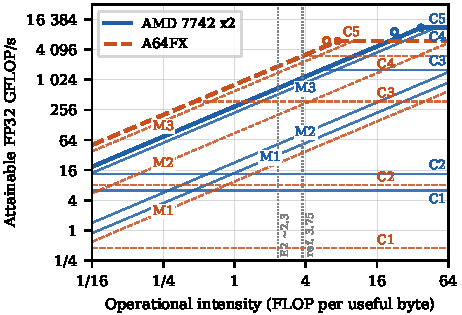
\includegraphics[width=0.62\linewidth]{roofline.pdf}
\caption{O roofline medido do AMD (azul) e do A64FX (laranja). As linhas grossas são o telhado e as
finas são os tetos. Os pontos cheios são os ridges medidos e os ocos os nominais. As linhas a ponteado
marcam a OI da referência (3.75) e da estratégia E2 ($\sim$2.3).}
\end{figure}

\subsection{O que o gráfico diz}
\begin{itemize}
\item \textbf{Ridge.} O do AMD passa de 22.5 (teórico) para 38 FLOP/B (medido), e o do A64FX de 6.0
para 7.4. No AMD isto acontece por duas razões: o clock real sobe o pico 22\% e a DDR4 só entrega 73\%
da banda teórica.
\porque{Um ridge mais à direita quer dizer que é preciso mais contas por byte para deixar de esperar pela
memória. O AMD é ``faminto'' de banda: quase tudo o que fizermos lá será limitado pela memória.}
\item \textbf{Na OI da referência (3.75)} as duas máquinas estão do lado da memória. Pelo roofline
simples, uma versão \emph{paralela} com a aritmética da referência (a E1) ficaria em 0.84 TFLOP/s no AMD
e 2.3 no A64FX com stores normais (teto M3), ou 1.1 e 3.0 sem write-allocate (M4, o telhado grosso do
gráfico). O A64FX tem só 54\% do pico do AMD, mas 2.7$\times$ a banda.
\porque{As contas: $3.75\times224=840$ GFLOP/s e $3.75\times606=2272$ (M3); $3.75\times299=1121$ e
$3.75\times813=3049$ (M4). Antes o texto dava os números do M3 sem dizer, e quem olhasse para o
gráfico (que desenha o M4) via 1.1 e 3.0.}
\cuidado{Este é só o limite da \emph{memória}. No A64FX as 7 divisões por ponto limitam a E1 a
2.2 Gpontos/s $\times$ 45 FLOP $\approx$ 0.1 TFLOP/s, 23$\times$ abaixo do M3 (secção seguinte). Antes o
relatório dizia ``memory bound a 2.3 TFLOP/s'' numa secção e ``limitada pelas divisões'' na outra: era
uma contradição (D28). A referência, sequencial e com stride, fica ainda mais abaixo.}
\end{itemize}

\section{1.3 Os tetos}\label{sec:tetos}
\subsection{A ideia}
O telhado é o melhor caso. Os \textbf{tetos} são linhas abaixo dele que mostram o limite quando o código
não usa alguma capacidade da máquina, por exemplo vetores, threads ou memória bem colocada. Estão
ordenados de baixo (o que a referência tem) para cima (o que exige mais esforço), como no artigo de
Williams.

\begin{table}[H]\centering\small
\caption{Os tetos, de baixo para cima (medidos; M1 e o M4 do AMD são calculados)}
\begin{tabular}{@{}llrr@{}}\toprule
 & \textbf{Teto e porque se aplica ao varcoef} & \textbf{AMD} & \textbf{A64FX} \\ \midrule
C1 & 7 divisões por ponto, escalar, 1 thread (a referência) & 6.2 & 0.44 \\
C2 & escalar, 1 thread, sem divisões (E2 + recíproco) & 13.5 & 8.0 \\
C3 & escalar, todos os cores (OpenMP) & 1589 & 379 \\
C4 & vetorial (SIMD) sem FMA & 10\,536 & 3022 \\
C5 & vetorial + FMA (pico) & 11\,269 & 6049 \\ \midrule
M1 & stride de um plano (ordem de ciclos da referência) & 14 & 9.5 \\
M2 & NUMA errado: toda a memória no nó 0 & 22.6 & 87.7 \\
M3 & com write-allocate (STREAM Triad) & 224 & 606 \\
M4 & sem write-allocate & 299 & 813 \\ \bottomrule
\end{tabular}\\[2pt]
\footnotesize C em GFLOP/s, M em GB/s.
\end{table}

\subsection{Tetos de cálculo}
\textbf{C1, as divisões: o teto mais importante para o varcoef.}
\begin{itemize}
\item \textbf{AMD (Zen 2):} uma divisão vetorial (\texttt{vdivps}, 8 floats) sai a cada 3.5 ciclos.
Medimos isto, e bate com o uops.info. É 14$\times$ abaixo do pico.
\item \textbf{A64FX:} uma divisão SVE (16 floats) tem latência de \textbf{98 ciclos} e é
\emph{bloqueante}: a seguinte só começa quando esta acaba. A divisão escalar demora 29 ciclos. Isto vem
do manual da Fujitsu, Tables 16-2 e 16-3, e põe as divisões \textbf{393$\times$} abaixo do pico.
\end{itemize}
\textbf{Como se chega a C1 $=$ 6.2 e 0.44 (D23).} Medimos quantas divisões escalares por segundo 1
thread faz: 0.9635 G/s no AMD e 0.0686 G/s no A64FX. Cada ponto tem 7 divisões e 45 FLOP, e as outras
38 operações correm em paralelo noutras unidades. Logo, o teto é
$0.9635\times45/7 = 6.2$ e $0.0686\times45/7 = 0.44$ GFLOP/s.
\cuidado{É um limite \emph{superior}: a referência divide em double, que é ainda mais lento.}

\textbf{Consequências em pontos por segundo:}
\begin{itemize}
\item A referência no A64FX (1 thread, escalar) chega no máximo a $2.0\text{ GHz}/(7\times29) = 9.9$
milhões de pontos por segundo.
\item Mesmo uma versão com 48 cores e SVE que mantenha as 7 divisões (E1) fica em cerca de 2.2 mil
milhões de pontos por segundo. Isto é 23$\times$ abaixo do que a HBM conseguiria alimentar.
\item No AMD, as divisões vetoriais ficam acima do teto da memória, por isso lá não são o problema.
\end{itemize}
\porque{O roofline simples, só com o pico FMA, não ``vê'' o custo das divisões: pela OI, a referência
parecia boa. É por isso que o C1 existe, e é por isso que a estratégia \textbf{E2} faz sentido. Com 4
materiais só há $4\times4 = 16$ valores possíveis de $\kappa_{pq}$, que cabem numa tabela na L1. Assim
eliminam-se as 6 divisões harmónicas.}
\cuidado{No A64FX, a E2 ainda fica limitada pela divisão final: cerca de 15 mil milhões de pontos por
segundo, 4$\times$ abaixo da HBM. Para lá chegar é preciso trocar a divisão por uma recíproca aproximada
(\texttt{FRECPE} com passos de Newton).}

\textbf{C2 e C3} correspondem a tirar as divisões e usar todos os cores. O C2 foi medido com FMAs
escalares, sem nenhuma divisão; a E2 ainda tem 1 divisão final, por isso no A64FX só chega ao C2 se essa
divisão também for trocada pelo recíproco (D28). \textbf{C4} é o teto sem FMA,
e quer dizer coisas diferentes em cada máquina:
\begin{itemize}
\item \textbf{Zen 2:} tem unidades separadas de MUL/FMA e de ADD, por isso sem FMA perde pouco (fica a
93\%).
\item \textbf{A64FX:} cada unidade faz FMA \emph{ou} MUL \emph{ou} ADD, por isso sem FMA perde metade.
\end{itemize}
\textbf{C5} (o pico) só é parcialmente atingível: a soma pesada encaixa em FMAs, o resto não.

\subsection{Tetos de memória}
\begin{itemize}
\item \textbf{M1, stride:} com a ordem de ciclos errada, cada leitura traz uma linha inteira e usa 4
bytes. No AMD a linha tem 64 B e só se usa 1/16; no A64FX tem 256 B e só se usa 1/64. Daí
$224/16 = 14$ e $606/64 = 9.5$ GB/s.
\cuidado{Uma só thread tira só 22 GB/s (AMD) ou 50 GB/s (A64FX) da memória. Com o stride, a referência
sequencial fica com 1.4 e 0.8 GB/s, muito abaixo do M1 do nó.}
\item \textbf{M2, NUMA errado:} corremos o STREAM com \texttt{numactl --membind=0}, que é o que acontece
quando uma só thread inicializa os arrays (``first touch''). A banda caiu 9.8$\times$ no AMD e
6.9$\times$ no A64FX. Ficou até abaixo do que um nó dá aos seus próprios cores, porque as threads dos
outros nós somam a latência do caminho e a contenção.
\porque{O Linux põe cada página no nó NUMA da thread que lhe escreveu primeiro. Por isso, na Task 2,
\textbf{a inicialização tem de ser paralela}, com o mesmo escalonamento OpenMP do cálculo.}
\item \textbf{M3 e M4, write-allocate:} um store normal primeiro \emph{lê} a linha para a cache e só
depois a escreve. O STREAM conta 24 B por elemento, mas na realidade movem-se 32 B. A prova está nos
números:
\begin{itemize}
\item no A64FX, o \texttt{zfill} (que evita a leitura) ganha 34\%, que é exatamente $32/24$;
\item no AMD, o Copy dá 298 GB/s. Se tivesse write-allocate, moveria $298\times24/16=447$ GB/s, mais do
que os 409.6 teóricos, o que é impossível.
\end{itemize}
\end{itemize}
A ordem M1 $<$ M2 $<$ M3 $<$ M4 confirma-se nas duas máquinas.

\section{1.4 Como vamos medir na Task 2}
\subsection{Protocolo}
\begin{itemize}
\item \textbf{Nós exclusivos:} ninguém partilha o nó connosco.
\item \textbf{Módulos com versão explícita}, registados em cada job juntamente com o clock e o governor.
\porque{Na Task 1 os scripts pediam o GCC 13.3, mas correu o 15.2 (os módulos numactl e OpenBLAS
trocam-no). Isso estraga a reprodutibilidade (D22).}
\item \textbf{Threads fixas} aos cores (\texttt{OMP\_PLACES=cores}).
\item \textbf{Compiladores:} GCC 15.2, mais o \texttt{fcc} da Fujitsu no A64FX e o \texttt{nvcc} na A100.
\item \textbf{Repetições:} 1 aquecimento e 10 repetições, com mediana e IQR.
\item \textbf{Ciclos com \texttt{perf stat}} em todos os testes de escalabilidade.
\item \textbf{Tempo sem profiler}, porque o profiler atrasa o código; os contadores medem-se numa
execução à parte.
\item \textbf{Validação:} cada versão é comparada com a saída da referência, e há sempre um teste curto
na partição \texttt{dev} antes de cada job longo.
\end{itemize}

\subsection{Profilers}
\begin{itemize}
\item \textbf{\texttt{perf} e PAPI:} existem nos dois CPUs, por isso os números comparam-se de forma
justa.
\item \textbf{\texttt{fapp}} no A64FX (uso do SVE, energia), que fica disponível depois de
\texttt{ml FJSVstclanga}.
\item \textbf{Nsight Systems/Compute} na A100.
\item \textbf{Energia:} RAPL via \texttt{perf} no AMD, \texttt{fapp} no A64FX e NVML na A100.
\end{itemize}
\cuidado{Tirámos o AMD uProf (o módulo não existe no Deucalion) e a energia do Slurm (o \texttt{sacct}
devolve 0).}

\subsection{Testes T1 a T10}
\begin{table}[H]\centering\small
\begin{tabular}{@{}l>{\raggedright}p{0.52\linewidth}>{\raggedright\arraybackslash}p{0.34\linewidth}@{}}\toprule
\textbf{Teste} & \textbf{O que mede} & \textbf{O que esperamos} \\ \midrule
T1 & Referência com 1 thread: tempo, MLUP/s, GFLOP/s, IPC & perto do C1 e do M1 de 1 thread \\
T2 & Escalabilidade forte (Amdahl) até 128/48 threads (tamanhos LLC-nó e RAM): speedup e fração série (Karp-Flatt) & satura quando a banda satura \\
T3 & Escalabilidade fraca (Gustafson) & tempo constante se a banda escalar \\
T4 & NUMA: first touch série vs paralelo, close vs spread & até 7--10$\times$ (M2) \\
T5 & Vetorização ligada/desligada, GCC vs fcc & ganho maior no A64FX \\
T6 & Misses e bytes da DRAM, para ter a OI medida & efeito da ordem dos ciclos \\
T7 & Overhead paralelo: barreiras e redução do resíduo & custo do resíduo \\
T8 & Energia: J até à solução, J/ponto, GFLOP/s/W & comparar as partições \\
T9 & A100: tempo do kernel, cópias, ocupação; Amdahl heterogéneo (Hill e Marty, 2008) & banda vs 1274 GB/s \\
T10 & Referência e melhor versão nos dois rooflines & distância aos tetos \\ \bottomrule
\end{tabular}
\end{table}

\porque{(D28) O enunciado pede, logo no Context, a lei de Amdahl em plataformas multicore heterogéneas
e a extensão de Gustafson. A lei de Amdahl diz que, se uma fração $s$ do trabalho é série, o speedup com
$p$ cores nunca passa de $1/(s+(1-s)/p)$. A métrica de Karp-Flatt faz a conta ao contrário: a partir do
speedup medido estima $s$. Se $s$ cresce com $p$, o problema não é código série, é a banda a saturar.
Hill e Marty (2008) aplicam Amdahl a chips com núcleos diferentes, que é o caso CPU + GPU do T9.
Gustafson (T3) responde à pergunta oposta: o que acontece se o problema crescer com os cores.}

\subsection{Tamanhos (D15, D22 e D28)}
Com 12 B por ponto numa grelha $(n+2)^3$ (o $+2$ é a borda), cada tamanho isola um nível de memória:
\begin{itemize}
\item \textbf{L1:} $n=11$ no AMD (25.7 de 32 KiB) e $n=14$ no A64FX (48 de 64 KiB; $n=15$ ficava
demasiado apertado para uma cache 4-way).
\item \textbf{LLC-1t (1 thread):} metade da LLC que uma thread vê, ou seja $n=86$ (7.8 MiB) no AMD e
$n=68$ (3.9 MiB) no A64FX.
\item \textbf{LLC-nó (todas as threads):} $n=250$ (183 MiB, 1.4 MiB por thread) no AMD e $n=110$
(16 MiB, 4 MiB por CMG) no A64FX.
\porque{Com $n=86$ e 128 threads, cada thread ficaria com 61 KiB, que cabem na L2 privada de 512 KiB. O
teste ``LLC'' estaria a medir a L2 sem darmos conta.}
\item \textbf{RAM:} $n=520$ nas três, que dá 1.59 GiB (1.19 GiB se o material passar a 1 byte).
É mais do que 1 GiB, como pede o enunciado, e não é potência de 2, o que evita conflitos de cache.
\item \textbf{A100 (Task 2.5):} LLC $n=110$ (16 MiB) e RAM $n=520$.
\porque{A L2 da A100 tem 40 MiB, mas são 2 metades de 20 MiB e a metade ``longe'' tem o dobro da
latência (medimos isso). 16 MiB cabem numa metade. O $n=250$ do AMD (183 MiB) não cabia.}
\cuidado{O check-up externo dizia que $n=14$ no A64FX causa conflitos de cache, porque cada array tem
$16^3\times4$ B = 16 KiB, exatamente o tamanho de uma ``via'' da L1 (64 KiB / 4 vias). A conta está
certa, a conclusão não: cada array de 16 KiB passa uma vez por cada um dos 64 conjuntos, e os 3 arrays
ocupam 3 das 4 vias de cada conjunto. Cabe tudo. O aliasing só faz mal quando há \emph{mais} endereços
no mesmo conjunto do que vias. Mantivemos $n=14$ (D28).}
\end{itemize}

\section{Para estudar antes da apresentação}
Perguntas que o professor pode fazer, com a resposta curta:
\begin{enumerate}
\item \textbf{Porque é que o pico medido do AMD é maior do que o teórico?} Porque o clock real sob carga
(2.81 GHz) é maior do que a base (2.25 GHz).
\item \textbf{Porque é que a referência tem OI alta e mesmo assim é lenta?} Por causa das divisões (C1)
e do stride (M1). A OI só diz quanto cálculo há por byte, não quanto custa cada operação.
\item \textbf{Porque é que o teto sem FMA é diferente nas duas máquinas?} Porque o Zen 2 tem unidades
de ADD separadas e o A64FX não tem.
\item \textbf{O que é o write-allocate e como sabemos que existe?} É a leitura da linha antes da
escrita. Sabemo-lo porque o zfill ganha exatamente $32/24$ e porque o Copy sem write-allocate não pode
ultrapassar a banda teórica.
\item \textbf{Porque é que a inicialização tem de ser paralela?} Por causa do first touch: com tudo num
nó NUMA, a banda cai 7 a 10$\times$.
\item \textbf{Porque usamos a mediana?} Porque os tempos têm outliers que puxam a média.
\end{enumerate}

\end{document}
